  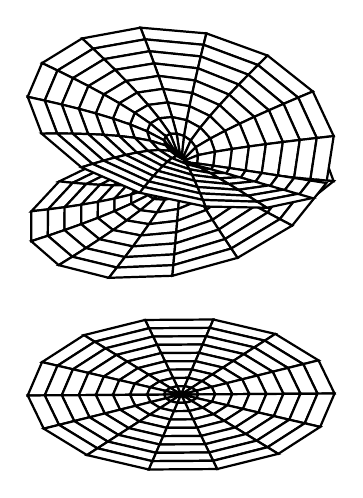
\begin{tikzpicture}[scale=2]
  \begin{axis}[
    axis equal image,
    axis lines=none,
    trig format plots=rad,
    z buffer=sort,
  ]

  \addplot3 [
    surf,
    domain=0:2*pi,
    samples=15,
    y domain =0:4,
    samples y=10,
    shader=flat,
    draw=black,
    fill=white,
  ]
  ({y*cos(x)}, {y*sin(x)}, {-7});

  \addplot3 [
    surf,
    shader=flat,
    draw=black,
    fill=white,
    z buffer=sort,
    domain=pi:5*pi,
    y domain = 0:4,
    samples = 30,
    samples y=10,
    ] 
  ({y*cos(x)}, {y*sin(x)}, {sqrt(y)*sin(x/2)});

  \end{axis}
  \end{tikzpicture}


